\documentclass[handout]{beamer}
\usepackage{multicol}
\usepackage{xy}
\everymath{\displaystyle}
\mode<presentation>
{\usetheme{Warsaw}\setbeamercovered{dynamic}}
\usecolortheme{crane}
\usepackage{beamerfoils}
\pgfdeclareimage[height=1in]{university-logo}{ISULogo}
\logo{\pgfuseimage{university-logo}}
\setbeamertemplate{navigation symbols}{}
\title[Craps]{Craps}
\author{Dr Marcus Bishop}
\subject{Math 104}
\beamerdefaultoverlayspecification{<+->}
\theoremstyle{definition}
\newtheorem{remark}{Remark}
\newtheorem{impact}{Impact}
\newtheorem{notation}{Notation}
\newtheorem{argument}{Argument}
\usepackage{arev}
\begin{document}
\begin{frame}\titlepage\end{frame}
\LogoOff

\begin{frame}{Two dice}
\begin{itemize}
\item Since rolling die has $6$ outcomes, rolling
two die has $6\cdot 6=36$ outcomes
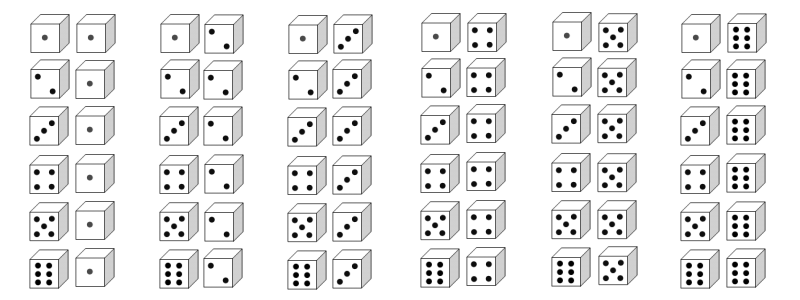
\includegraphics{TwoDice}
\item Rolling two dice and adding has $11$ outcomes,
namely $2,3,\ldots,12$
\item[]
\[\begin{array}{r|c|c|c|c|c|c|c|c|c|c|c}
\text{Sum}&2&3&4&5&6&7&8&9&10&11&12\\\hline
\text{Frequency}&\only<+->{1}&
\only<+->{2}& \only<+->{3}& \only<+->{4}& \only<+->{5}&
\only<+->{6}& \only<+->{5}& \only<+->{4}& \only<+->{3}&
\only<+->{2}& \only<+->{1} \end{array}\]
\end{itemize}
\end{frame}

\begin{frame}{Craps}
\begin{itemize}
\item Each player chooses to be either a \alert{pass bettor}
or a \alert{don't pass bettor}
\item \alert{Shooter} rolls two dice
\item If $7$ or $11$ the sum (a \alert{natural}) then pass bettors win (and don't pass bettors lose)
\item If $2$, $3$, or $12$ the sum (a \alert{craps})
then don't pass bettors win (and pass bettors lose)
\item If $4,5,6,8,9,10$ the sum,
then this number called \alert{the point}
\item Shooter rolls dice until sum is either $7$ or the point
\item If point occurs first, then pass bettors win (\alert{point is made})
\item If $7$ occurs first, then don't pass bettors win
\item Game continues as above, with dice rolled by same shooter
until point established and fails to be made
\end{itemize}
\end{frame}

\begin{frame}
\begin{itemize}
\item Want to calculate expected proceeds for pass bettors
\item Need to enumerate all possible outcomes and find probability of each
\[\begin{xy}<1.4cm,0cm>:
(4.5,0)="0"; (1,-2)="N"; (2,-2)="C"; (3,-2)="4";
(4,-2)="5"; (5,-2)="6"; (6,-2)="8"; (7,-2)="9"; (8,-2)="10";
"0";"N"*+!D{N}**\dir{-};
"0";"C"*+!D{C}**\dir{-};
"0";"4"*+!D{4}**\dir{-};
"0";"5"*+!D{5}**\dir{-};
"0";"6"*+!D{6}**\dir{-};
"0";"8"*+!D{8}**\dir{-};
"0";"9"*+!D{9}**\dir{-};
"0";"10"*+!D{10}**\dir{-};
"4";(2.75,-4)*+!D{P}**\dir{-};
"4";(3.25,-4)*+!D{F}**\dir{-};
"5";(3.75,-4)*+!D{P}**\dir{-};
"5";(4.25,-4)*+!D{F}**\dir{-};
"6";(4.75,-4)*+!D{P}**\dir{-};
"6";(5.25,-4)*+!D{F}**\dir{-};
"8";(5.75,-4)*+!D{P}**\dir{-};
"8";(6.25,-4)*+!D{F}**\dir{-};
"9";(6.75,-4)*+!D{P}**\dir{-};
"9";(7.25,-4)*+!D{F}**\dir{-};
"10";(7.75,-4)*+!D{P}**\dir{-};
"10";(8.25,-4)*+!D{F}**\dir{-};
\end{xy}\]
\end{itemize}
\end{frame}

\begin{frame}
\begin{itemize}
\item $P\left(N\right)=
P\left(\text{$7$ or $11$}\right)
=\frac{6}{36}+\frac{2}{36}=\frac{8}{36}$
since $7$ and $11$ mutually exclusive
\[\begin{xy}<1.4cm,0cm>:
(4.5,0)="0";
(1,-2)="N";(2,-2)="C";(3,-2)="4";(4,-2)="5";
(5,-2)="6";(6,-2)="8";(7,-2)="9";(8,-2)="10";
"0";"N"*+!D{N}**\dir{-}?*+!R{\alert{\frac{8}{36}}};
"0";"C"*+!D{C}**\dir{-};
"0";"4"*+!D{4}**\dir{-};
"0";"5"*+!D{5}**\dir{-};
"0";"6"*+!D{6}**\dir{-};
"0";"8"*+!D{8}**\dir{-};
"0";"9"*+!D{9}**\dir{-};
"0";"10"*+!D{10}**\dir{-};
"4";(2.75,-4)*+!D{P}**\dir{-};
"4";(3.25,-4)*+!D{F}**\dir{-};
"5";(3.75,-4)*+!D{P}**\dir{-};
"5";(4.25,-4)*+!D{F}**\dir{-};
"6";(4.75,-4)*+!D{P}**\dir{-};
"6";(5.25,-4)*+!D{F}**\dir{-};
"8";(5.75,-4)*+!D{P}**\dir{-};
"8";(6.25,-4)*+!D{F}**\dir{-};
"9";(6.75,-4)*+!D{P}**\dir{-};
"9";(7.25,-4)*+!D{F}**\dir{-};
"10";(7.75,-4)*+!D{P}**\dir{-};
"10";(8.25,-4)*+!D{F}**\dir{-};
(1,-4)*+!U{\alert{\frac{2}{9}}};
\end{xy}\]
\end{itemize}
\end{frame}

\begin{frame}
\begin{itemize}
\item Want to calculate $P\left(\text{$4$ and $P$}\right)$
\item $3$ ways to roll $4$ so $P\left(4\right)=\frac{3}{36}$
\item Assume $4$ occurs
\item $3$ ways to roll $4$ again (point is made, pass
bettors win, denoted by \alert{$P$} in tree)
\item $6$ ways to roll $7$ (point not made, don't pass
bettors win, denoted by \alert{$F$} in tree)
\item Outcomes other than $4$ and $7$ ignored
\item So $9$ possible outcomes
\item Thus $P\left(P\right)=\frac{3}{9}$
and $P\left(F\right)=\frac{6}{9}$
\item Therefore
$P\left(\text{$4$ and $P$}\right)
=\frac{3}{36}\cdot\frac{3}{9}=\frac{1}{36}$
\item Similarly $P\left(\text{$4$ and $F$}\right)
=\frac{3}{36}\cdot\frac{6}{9}=\frac{1}{18}$
\end{itemize}
\end{frame}

\begin{frame}
\[\begin{xy}<1.4cm,0cm>:
(4.5,0)="0";
(1,-2)="N";(2,-2)="C";(3,-2)="4";(4,-2)="5";
(5,-2)="6";(6,-2)="8";(7,-2)="9";(8,-2)="10";
"0";"N"*+!D{N}**\dir{-}?*+!R{\frac{8}{36}};
"0";"C"*+!D{C}**\dir{-};
"0";"4"*+!D{4}**\dir{-}?*{\alert{\frac{3}{36}}};
"0";"5"*+!D{5}**\dir{-};
"0";"6"*+!D{6}**\dir{-};
"0";"8"*+!D{8}**\dir{-};
"0";"9"*+!D{9}**\dir{-};
"0";"10"*+!D{10}**\dir{-};
"4";(2.75,-4)*+!D{P}**\dir{-}?*{\alert{\frac{3}{9}}};
"4";(3.25,-4)*+!D{F}**\dir{-}?*{\alert{\frac{6}{9}}};
"5";(3.75,-4)*+!D{P}**\dir{-};
"5";(4.25,-4)*+!D{F}**\dir{-};
"6";(4.75,-4)*+!D{P}**\dir{-};
"6";(5.25,-4)*+!D{F}**\dir{-};
"8";(5.75,-4)*+!D{P}**\dir{-};
"8";(6.25,-4)*+!D{F}**\dir{-};
"9";(6.75,-4)*+!D{P}**\dir{-};
"9";(7.25,-4)*+!D{F}**\dir{-};
"10";(7.75,-4)*+!D{P}**\dir{-};
"10";(8.25,-4)*+!D{F}**\dir{-};
(1,-4)*+!U{\frac{2}{9}};
(2.75,-4)*+!U{\alert{\frac{1}{36}}};
(3.25,-4)*+!U{\alert{\frac{1}{18}}};
\end{xy}\]
\end{frame}

\end{document}

\begin{frame}{Homework for Monday 6 October}
\begin{itemize}
\item Print or otherwise reproduce slide 28
\item Calculate probability of remaining outcomes,
writing them directly on tree
\item Verify that $1$ the sum of probabilities
of all outcomes
\item Assuming that pass bettors and
don't pass bettors each bet $100$,
calculate expected proceeds for both groups.
\item Also complete exercises 15--34 of textbook
\end{itemize}
\end{frame}

\begin{frame}{Probabilities of all winning outcomes}
\begin{itemize}
\item $P\left(N\right)=2/9$ (calculation above)
\item $P\left(\text{$4$ and $P$}\right)=1/36$ (calculation above)
\item $P\left(\text{$5$ and $P$}\right)=\frac{4}{36}\cdot\frac{4}{10}
=\frac{2}{45}$
\item $P\left(\text{$6$ and $P$}\right)=25/396$
\item $P\left(\text{$8$ and $P$}\right)=25/396$
\item $P\left(\text{$9$ and $P$}\right)=2/45$
\item $P\left(\text{$10$ and $P$}\right)=1/36$
\item So pass bettors win $\$100$ with probability
\[\frac{2}{9}+2\left(\frac{1}{36}\right)
+2\left(\frac{2}{45}\right)+2\left(\frac{25}{396}\right)
=\frac{244}{495}\approx 0.4929\]
\end{itemize}
\end{frame}

\begin{frame}{Probabilities of all losing outcomes}
\begin{itemize}
\item $P\left(C\right)=\frac{4}{36}=\frac{1}{9}$
\item $P\left(\text{$4$ and $F$}\right)=1/18$ (calculation above)
\item $P\left(\text{$5$ and $F$}\right)=\frac{4}{36}\cdot\frac{6}{10}
=\frac{1}{15}$
\item $P\left(\text{$6$ and $F$}\right)=5/66$
\item $P\left(\text{$8$ and $F$}\right)=5/66$
\item $P\left(\text{$9$ and $F$}\right)=1/15$
\item $P\left(\text{$10$ and $F$}\right)=1/18$
\item So pass bettors lose $\$100$ with probability
\[\frac{1}{9}+2\left(\frac{1}{18}\right)
+2\left(\frac{1}{15}\right)+2\left(\frac{5}{66}\right)
=\frac{251}{495}\approx 0.507\]
\end{itemize}
\end{frame}

\begin{frame}{Craps expectation}
\begin{itemize}
\item Observe that $\frac{244}{495}+\frac{251}{495}=1$
\item Expected proceeds for pass bettors:
\[100\left(\frac{244}{495}\right)-100\left(\frac{251}{495}\right)
=-\frac{140}{99}\approx \$-1.41\]
\item Expected proceeds for don't pass bettors:
\[-100\left(\frac{244}{495}\right)+100\left(\frac{251}{495}\right)
=\frac{140}{99}\approx \$1.41\]
\end{itemize}
\end{frame}

\begin{frame}{Casino craps}
\begin{itemize}
\item In casino, payouts for pass bettors the same as in street version
\item So pass bettors win amount bet
for favorable outcomes: $N$,
$\left(\text{$4$ and $P$}\right)$,\dots,
$\left(\text{$12$ and $P$}\right)$
\item Thus $\$-1.41$ the expectation for pass bettors
for every $\$100$ bet
\item However, if initial roll results in $12$, don't pass bettors
neither win nor lose
\item Thus outcome $C$ splits into two outcomes for don't pass bettors:
\begin{itemize}
\item Don't pass bettors win amount bet if first roll $2$ or $3$
\item Don't pass bettors win $0$ if first roll $12$
\end{itemize}
\end{itemize}
\end{frame}

\begin{frame}
\begin{itemize}
\item Recall that expected proceeds for don't pass bettors
in \alert{street} version:
\[-100\left(\frac{244}{495}\right)+100\left(\alert{\frac{251}{495}}\right)
=\frac{140}{99}\approx \$1.41\]
\item Here
\[\frac{251}{495}
=\alert{\frac{1}{9}}+2\left(\frac{1}{18}\right)
+2\left(\frac{1}{15}\right)+2\left(\frac{5}{66}\right)\]
\item Here $\frac{1}{9}=\frac{4}{36}$ the probability of $C$
\item In \alert{casino} version, change $\frac{1}{9}$ to
$\frac{3}{36}=\frac{1}{12}$, the probability of $2$ or $3$
\end{itemize}
\end{frame}

\begin{frame}
\begin{itemize}
\item Thus outcome $\$100$ occurs with probability
\[\alert{\frac{1}{12}}+2\left(\frac{1}{18}\right)
+2\left(\frac{1}{15}\right)+2\left(\frac{5}{66}\right)
=\frac{949}{1980}\approx 0.4793\]
\item Thus expectation for don't pass bettors
\[-100\left(\frac{244}{495}\right)+100\left(\alert{\frac{949}{1980}}\right)
+\alert{0\left(\frac{1}{36}\right)}
=-\frac{15}{11}\approx \$-1.37\]
\item Thus expectation for pass bettors $\$-1.41$
close to expectation for don't pass bettors
\end{itemize}
\end{frame}

\begin{frame}{Chuck-a-luck}
\begin{multicols}{2}
\begin{itemize}
\item Chuck-a-luck popular in carnivals, less
popular in casinos
\item Played with three regular dice
\item Players bet on one of $1,2,\ldots,6$
\item Dealer rolls three dice
\item House pays player amount bet for every
die showing chosen number
\item However, if no die shows chosen number,
house keeps bet
\end{itemize}
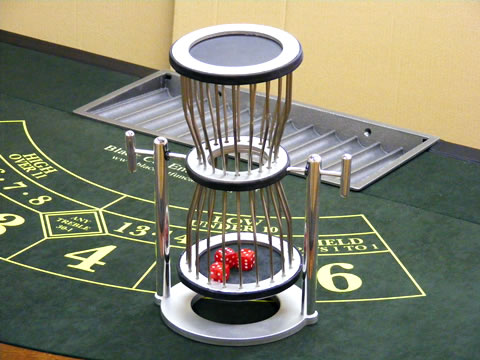
\includegraphics[scale=.35]{Chuck}
\end{multicols}
\end{frame}

\begin{frame}
\begin{example}
\begin{itemize}
\item Suppose player bets $\$1$ on number $3$
\item If dice show $3,1,6$ player wins $\$1$
\item If dice show $1,3,3$ player wins $\$2$
\item If dice show $1,5,2$ player loses $\$1$
\end{itemize}
\end{example}
\begin{center}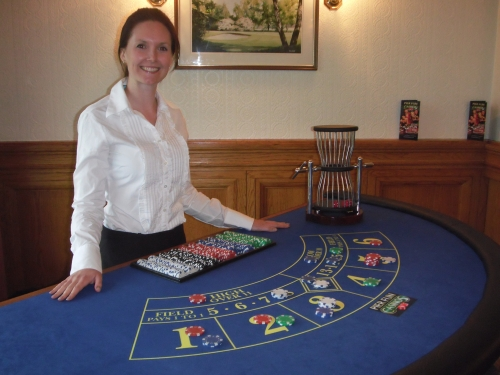
\includegraphics[scale=.35]{Chuck2}\end{center}
\end{frame}

\begin{frame}
Chuck-a-luck seems attractive by following \alert{incorrect} argument
\begin{argument}
\begin{itemize}
\item Suppose $1$ the chosen number (for concreteness)
\item Let $E_1$ be event that first die shows $1$
\item Let $E_2,E_3$ be events that second, third dice show $1$
\item Then $P\left(E_1\right)=P\left(E_2\right)=P\left(E_3\right)
=\frac{1}{6}$
\item So $P\left(\text{$E_1$ or $E_2$ or $E_3$}\right)
=\frac{1}{6}+\frac{1}{6}+\frac{1}{6}=\frac{1}{2}$
the probability that at least one die shows $1$
\item Thus game is at least fair
\item Furthermore, possibility of \alert{multiple} dice
showing $1$ further increases chances of winning
\end{itemize}
\end{argument}
But $E_1,E_2,E_3$ \alert{not mutually exclusive}!
\end{frame}

\begin{frame}{Chuck-a-luck probabilities}
\begin{itemize}
\item $216=6^3$ the number of possible outcomes
\item $1,1,1$ occurs in only one way, so $\frac{1}{216}$
the probability of $1,1,1$
\item Two $1$'s occurs in five ways as $1,1,x$
where $x\ne 1$
\item Can also occur in further five ways as $1,x,1$
and still further five ways as $x,1,1$
\item So $\frac{15}{216}$ the probability of two $1$'s
\item Single $1$ occurs as $1,x,y$ where $x,y\ne 1$
\item Occurs in $5\cdot 5=25$ ways
\item Single $1$ occurs in further $25$ ways as $x,1,y$
and still further $25$ ways as $x,y,1$
\item Thus $\frac{75}{216}$ the probability of single $1$
\end{itemize}
\end{frame}

\begin{frame}
\begin{itemize}
\item Note that $\frac{1}{216}+\frac{15}{216}+\frac{75}{216}
=\frac{91}{216}\approx 0.4213$ the probability of winning
\item Note that $0.4213<0.5$ so Chuck-a-luck \alert{not} fair!
\item Note that $1-\frac{91}{216}=\frac{125}{216}$
the probability of losing
\item If player bets $\$1$ then expectation
\begin{multline*}
3\left(\frac{1}{216}\right)
+2\left(\frac{15}{216}\right)+1\left(\frac{75}{216}\right)
-1\left(\frac{125}{216}\right)\\
=-\frac{17}{216}\approx \$-0.0787
\end{multline*}
\item So player expected to lose $7.87$ cents per dollar spent
in long run
\end{itemize}
\end{frame}

\end{document}
